\section{Evaluering}\label{sec:rtp_evalation}
Vi har i dette afsnit beskrevet hvad der skal til, for at implementere RTP i \pycsp. Vi vil i dette afsnit gennemgå hvordan RTP kan implementeres, for derefter at evaluere vores løsning med udgangspunkt i slagterieksemplet.
\subsection{Test af Korrekthed}
Vi har som i \des i \cref{sec:des-eval} løbende skrevet tests, før vi implementerede hver ny funktion i \code{RTP}-versionen.  Bilag \ref{app:rtp-test} viser testresultaterne for de tests der er lavet specifikt for \code{RTP}-versionen.

Alle tests undtagen én fungerer korrekt. Testen, der fejler hedder test"_xreset"_inheritance"_from"_two"_step og viser en situation, hvor den samme proces får løftet sin prioritet to gange i træk, først med en høj prioritet og efterfølgende med en mellemprioritet. Efterfølgende skal processen sænke sin prioritet, først til  mellemprioriteten og til slut til sin originale prioritet. Her viser det sig, at vi har lavet en fejl i implementeringen, således at prioriteten ikke bliver nedsat til mellemprioriteten. \CRef{fig:priority-inheritance} viser prioriteten, mens processen bliver op- og nedprioriteret. Vi har ikke prioriteret at løse dette problem, men det kan løses ved at kræve, at når en proces opprioriteres, gemmes oplysningen om, hvilken proces der står bag, så når en proces ønsker at fjerne sin opprioritering fra andre processer, er det kun sin egen  prioritet, den fjerner.  
 
  
\begin{figure}
 \begin{center}
  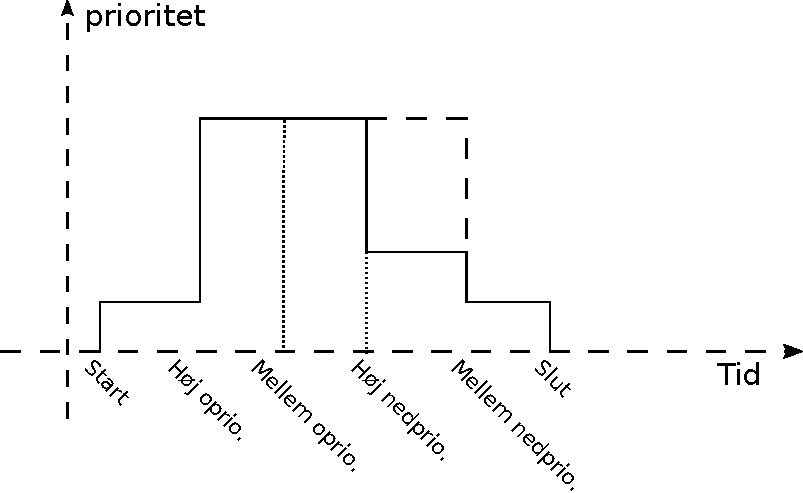
\includegraphics[scale=1]{images/priority-inheritance}
	\caption{Figuren viser hhv. forventet og faktisk prioritetsarvning. Der hvor den faktiske og forventede opførsel adskiller sig er forventet den fuldt optrukne streg, mens den stiplede streg er den faktiske opførsel.}
	\label{fig:priority-inheritance}
\end{center}
\end{figure}
  

\subsection{Slagterieksempel}
Vi vil nu sammenligne implementeringerne i de tre eksisterende versioner af \pycsp mod henholdsvis hinanden og \code{RTP}-versionen. Ud fra denne sammenligning vil vi se på fordele og ulemper ved de forskellige versioner.

Ved at benytte \pycsp til slagterieksemplet opnår man et modulært design, der nemt kan udvides hvis de fysiske rammer for slagteriet ændrer sig. Viser det sig f.eks at kameraet holder den samlede produktivitet af netværket tilbage, kan slagteriet nemt tilføje endnu et kamera, og udvide procesnetværket med endnu en kameraproces, som kan arbejde samtidigt med det første kamera. 

En kørsel af de tre eksisterende versioner giver et meget forskelligt resultat, som vist i \cref{tab:deadline-runs2}. I denne tabel har vi foretaget en simulering af 100 grise. Denne simulering er kørt 10 gange, og tabellen viser gennemsnittet og standardafvigelsen. Af tabellen kan man se at versionen som forventet har betydning for antallet af grise der rettidigt kan nå at blive bearbejdet. 

\code{Proces}-versionen er ikke som forventet bedre en de andre versioner til at bearbejde griseobjekterne rettidigt. Dette skyldes at testen er gennemført på en maskine, med kun en kerne.  Dermed kan \code{processes}-versionen ikke drage nytte  af flere kerner, men er begrænset til kun at kunne køre en proces af gangen. I \code{processes}-versionen, foregår kontekstskiftene i operativsystemets \sched, der er væsentligt langsommere end i \code{greenlets}- og \code{RTP}-versionen, hvor konktekstskiftene sker i vores \sched. 

I vores arbejde med anvendelsesområdet interaktiv planlægning i kapitel \ref{chap:is}, har vi implementeret et prioritetssystem for processer, da vi netop indenfor dette anvendelsesområde, har tænkt på det som en mulig udvidelse. Vi har derfor medtaget resultater hvor vi har højere prioriteter på de essentielle processer. Umiddelbart ser det ud til at forværre ydelsen, hvilket må tillægges at håndteringen af prioriteter skaber et overhead, sammenholdt med, at alle processer i denne version af eksemplet er lige vigtige. 


%\begin{table}[htbp]
%  \vspace{0.5cm}
%	\centering
%	\begin{tabular}{lcc}
%       	\toprule
%        \mc{Version}  &\mc{Succesrate (\%)}&\mc{Standard Afvigelse (SA)}\\
%        \midrule
%        Processes&1 & 1 \\
%        Threads & 14 & 7\\
%        Greenlets & 18& 9 \\        
%        RTP u. prioritet &22  &8 \\
%        RTP m. prioritet & 17 & 8\\
%        \bottomrule
%    \end{tabular}
%	\caption[]{10 kørsler hvor 100 grise bliver sendt igennem procesnetværket. }\\
%	\label{tab:deadline-runs}
%\end{table}

\begin{table}[htbp]
	\centering
	\begin{tabular}{lccc}
       	\toprule
        \mc{Version}  &\mc{Samtidige grise} & \mc{Succesrate (\%)} & \mc{Standard Afvigelse (SA)} \\
        \midrule
        Processes        & 1 & 16 & 2 \\
        Processes        & 2 &  0 & 0 \\
        Processes        & 3 &  0 & 0 \\
        Processes        & 5 &  0 & 0\\
        \midrule
        Threads          & 1 & 34 & 6 \\
        Threads          & 2 &  1 & 1 \\
        Threads          & 3 &  1 & 0 \\
        Threads          & 5 &  1 & 1 \\
        \midrule
        Greenlets        & 1 & 44 & 7 \\
        Greenlets        & 2 & 49 & 1 \\
        Greenlets        & 3 & 32 & 0\\
        Greenlets        & 5 & 20 & 0 \\
        \midrule
        RTP u. prioritet & 1 & 42 & 6 \\
        RTP u. prioritet & 2 & 44 & 2 \\
        RTP u. prioritet & 3 & 31 & 2 \\
        RTP u. prioritet & 5 & 19 & 0 \\
        \midrule
        RTP m. prioritet & 1 & 44 & 10\\
        RTP m. prioritet & 2 & 21 & 5\\
        RTP m. prioritet & 3 & 21 & 7\\
        RTP m. prioritet & 5 &  7 & 3\\

        \bottomrule
    \end{tabular}
	\caption[]{10 kørsler hvor 100 grise bliver sendt igennem procesnetværket. }\\
	\label{tab:deadline-runs2}
\end{table}

For at få mere samtidigt arbejde har vi ændret indstillingerne for simuleringen, så transportbåndet er længere, og dermed giver mere tid til at nå deadlinen, men samtidig har vi flere grise samtidigt i simuleringen. Resultaterne af dette fremgår af \cref{tab:deadline-runs2}. Når antallet af grise, der skal bearbejdes samtidigt stiger, øges antallet af processer, der må kæmper mod hinanden for CPU-tid. Dette er ens for de tre eksisterende versionerne af \pycsp.  

I \code{Proces}-versionen medfører det  muligheden for, at griseobjekterne kan blive  bearbejdet parallelt, hvis computeren har denne mulighed.  Ofte vil der være flere griseobjekterne end processorer, hvorfor griseobjekterne stadig vil skulle kæmpe mod hinanden, for at komme igennem netværket. Når griseobjekterne skal kæmpe for at komme igennem netværket, sker det, i denne version, uden hensyn til hvilken gris der er nærmest robotten. Man risikerer dermed en situation hvor griseobjekterne kan overhale hinanden, så det ikke er grisene nærmest robotten der først bliver bearbejdet.

\code{RTP}-udvidelsen bygger på \code{greenlets}-versionen, og vil derfor have de samme begrænsninger som denne, som diskuteret i implementeringen i afsnit \cref{sec:deadline-exampel-implementation}. Grisseobjekter kan ikke  på samme måde overhale hinanden i \code{RTP}-versionen, da hver proces har tilknyttet griseobjektets deadline. Dermed sikres, at det altid er griseobjektet tættest på sin deadline, der sendes igennem netværket først.

I \code{RTP}-versionen, slipper de enkelte processer desuden for at holde styr på tiden, og vurdere om det enkelte griseobjekts deadline, er overskredet. Når de starter, har de en deadline svarende til det tidspunkt robotten senest skal have griseobjektet. Denne sættes via funktionen \code{Set\_deadline}. \code{Set\_deadline} kan resultere i en exception, og derfor skal hver proces kunne håndtere en \code{DeadlineException}, som de i dette eksempel blot kan håndtere, ved at smide griseobjektet væk. Det kan de gøre, da robotten på dette tidspunkt tager sin beslutning, og derfor vælger at udskære grisen uden specialviden. Griseobjektet er dermed ikke længere relevant og kan smides væk, så processen kan gå i gang med modtage et nyt griseobjekt.

I \code{greenlets}-versionen kom vi ind på at processerne frivilligt skal afgive kontrollen, før robotten kan foretage udskæringen, men at der ikke findes en metode til midlertidigt at afgive kontrollen. Med \code{RTP}-versionen og funktionen \code{Release}, har alle processer mulighed for at afgive kontrollen, så robotten rettidigt kan foretage selve udskæringen. Hermed skal vi ikke introducere en delt datastruktur, men kan lade det være op til robotprocessen at igangsætte robotten.
  
%selvom det var nødvendigt at basere \code{RTP} på  \code{greenlets}-versionen medfører det, at kun en proces kan være aktiv af gangen. Dermed kan vi kun udnytte en processor, som  passer dårligt sammen med denne applikation, som det ses af \cref{tab:deadline-runs}.  Vi kan dog til dels afhjælpe dette problem ved at udnytte at der i \code{greenlets}-versionen, findes en \code{IO}-dekorering. Denne dekorering placerer en funktion i en separat tråd, så flere funktioner kan køre samtidigt. Man skal her dog være opmærksom på at GIL'en stadig forhindre parallel udførsel. Eventuel parallel udførsel vil derfor kræve at koden i IO dekoreringen, kalder eksterne moduler som diskuteret i \cref{chap:csp}. Denne mulighed for parallel bearbejdning af flere processer vil dog  som i \code{processes}-versionen resultere i at processerne vil kæmpe mod hinanden om CPU-resurser. \code{RTP}-versionen har dog den store fordel at vi, i modsætning til \code{proces}-versionen, ikke risikerer at griseobjekterne overhaler hinanden, men at netværket hele tiden har fokus på først at videresende griseobjektet nærmest robotten. \CRef{fig:pig-network3} viser hvordan netværket kan se ud med flere konverterings- og analyseprocesser.

%\begin{figure}
% \begin{center}
%  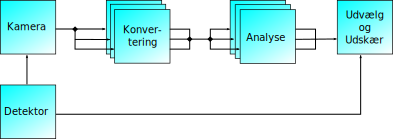
\includegraphics[scale=1]{images/pig-network3}
%	\caption{Procesnetværk med flere konverteringsprocesser, og analyseprocesser}
%	\label{fig:pig-network3}
%\end{center}
%\end{figure}


Efter at have implementeret \code{RTP}-versionen, og implementeret vores eksempel i denne version, kan vi i \cref{tab:deadline-runs2} se at vores løsning ikke er mærkbart bedre en \code{greenlets}-versionen. Dette mener vi skyldes, at det valgte eksempel er for simpelt og derfor ikke lader \code{RTP}-versionen komme til sin ret. I eksemplet har alle processer den samme deadline, i forhold til hvornår de ankommer, hvorfor de alle er lige begrænset. At udvælge et griseobjekt frem for et andet, har ikke indflydelse på  hvor mange griseobjekter vi i alt kan nå, men ændre blot hvilke af griseobjekterne, der bliver bearbejdet rettidigt. Det ekstra arbejde vi foretager i \sched en gavner ikke slagterieksemplet, men  begrænser tværtimod \code{RTP}-versionen i tiden processerne har til at bearbejde hvert griseobjekt.

Med udgangspunkt i at eksemplet ikke er optimalt til at vise vores løsning, ønsker vi at ændre eksemplet, for at se hvordan \code{RTP}-versionen bruges, hvis ikke alle processerne har en deadline. Vi har udvidet slagterieksemplet med en ekstra proces. Denne dummyproces har ingen deadline, og kører i en fast løkke, der estimerer $\pi$. Formålet med processen er at simulere et arbejde der også ønskes udført, men som ikke er tidskritisk. Når \code{greenlets}-versionen udvælger hvilke processer der skal køres, gøres det tilfældigt, hvorfor processen uden deadline kan risikere at blokere for de tidskritiske processer. I \code{RTP}-versionen bør tiden vi bruger i  dummyprocessen til gengæld begrænses, når der er tidskritiske processer, der skal bearbejdes.

Ved at introducere en dummyproces, oplevede vi indledningsvis at \code{greenlets}-versionen, ikke blev færdig, men befandt sig i en  livelock. Grunden til dette skyldtes  en blanding af vores implementering af dummyprocessen, og implementeringen af \code{greenlets}-versionen. Som det ses af \cref{dummy1}, bruger vi en \code{alternation} for midlertidigt at afgive kontrollen så den senere kunne genplanlægges, samt at detektere hvornår vi skal slutte, da kanalen så vil være blevet forgiftet.
Denne løsning placerer processen på \code{timers}listen, men da \sched en foretrækker, at planlægge processer fra denne liste frem for \code{next}-listen, og dummyprocessen altid er klar til at blive udvalgt, vil det kun være dummyprocessen der bliver bearbejdet. Det samme problem gør sig ikke gældende i \code{RTP}-versionen, da processer i \code{timers}-listen bliver planlagt på lige fod med alle andre processer.

\begin{lstlisting}[firstnumber=1,float=hbtp, label=dummy1, caption=Uddrag af Dummyproces]
while True:
    Alternation([{Timeout(seconds=0.005):None}, {dummy_in:None}]).select()
    time_spent -= time.time()
    dummywork(work)
    time_spent += time.time()          
\end{lstlisting}

For ikke unødigt at give vores version en fordel har vi valgt at ændre dummyprocessen, så også \code{greenlets}-versionen kan blive færdig. Vi har ikke mulighed for i \code{greenlets}-versionen manuelt at stoppe eksekveringen af processen, og lade den  blive placeret på \code{next}-listen. Den eneste måde for en proces at komme på denne liste er efter at have kommunikeret. Vi ændrer derfor dummyprocessen til et dummynetværk bestående af to processer, der hver foretager et stykke arbejde og kommunikerer, som vist i \cref{dummy2}. I dette netværk findes der to dummyprocesser, der skiftes til at sende hinanden den akkumulerede tid de har været aktive. Fordi de efter hver periode, sender den akkumulerede tid til den anden dummyproces, vil den ene hele tiden skulle vente, for så at blive lagt på \code{next}-listen. Dermed  indgår dummyprocesserne  på lige fod med alle andre aktive processer i netværket.

\begin{lstlisting}[firstnumber=1 ,float=hbtp, label=dummy2, caption=Uddrag Dummynetværk]
while True:
    time_spent = dummy_in()
    time_spent -= time.time()
    dummywork(work)
    time_spent += time.time()
    dummy_out(time_spent)  
\end{lstlisting}



\begin{table}[htbp]
	\centering
	\begin{tabular}{lcccc}
       	\toprule
        \mc{Version}&\mc{Tid i dummyproces(s)}&\mc{SA.}& \mc{Succesrate (\%)}&\mc{SA.}\\
        \midrule
        Greenlets         & 1.29 & 0.61 & 13 & 2  \\
        RTP               & 1.05 & 0.28 & 24 & 6  \\
        RTP m. prioritet  & 0.74 & 0.34 & 42 & 13 \\
        \bottomrule
    \end{tabular}
	\caption[]{10 * 100 grise køres igennem procesnetværket. Desuden er der tilknyttet en dummyproces, uden en deadline, der hele tiden ønsker at arbejde. For hver kørsel udregnes hvor meget kørselstid dummyprocessen har kørt, samt antallet af grise der bliver rettidigt bearbejdet.}\\
	\label{tab:dummy-run}
\end{table}

\CRef{tab:dummy-run} viser den gennemsnitlige tid hver version har brugt i dummyprocessen, samt hvor mange grise, der er blevet bearbejdet rettidigt. 
Som det ses, bruges der mindre tid i dummyfunktionen i \code{RTP}-versionen end i \code{greenlets}-versionen. Dette medfører at antallet af grise, der rettidigt bliver bearbejdet, er højere i \code{RTP}-versionen. Denne test viser dermed, at \code{RTP}-versionen formår at udvælge de tidskritiske processer, på bekostning af processer uden deadline, og at denne udvælgelse medfører en øget succesrate, på trods af den øgede kompleksitet i \code{RTP}-versionen. Vi ser yderligere at den ekstra funktionalitet til at håndtere prioritet spiller en stor rolle, når vi introducerer dummyprocesserne. Det sker fordi vi nu har en et scenarium, hvor vi kan differentiere i i prioriteten af de enkelte processer, og sikre at de højt prioriterede processer afvikles når der er brug for det.


